\section{Background}

In this section, we discuss the design of state-of-the art systems that provide
access to remote memory and storage. Specifically, in our study we use Network
Block Device (NBD) ~\cite{nbd}, NVMe over Fabrics (NVMe-oF) ~\cite{nvme-of}, and the Storage Performance
Development Kit (SPDK) ~\cite{spdk}.
\subsection{Network Block Device (NBD)}
 Network Block Device (NBD) is a network protocol that can be used to export a block device from a server where the block device resides to a client. Figure \ref{fig:nbd_path} shows an overview of an NBD system.
 \begin{figure}[h]
    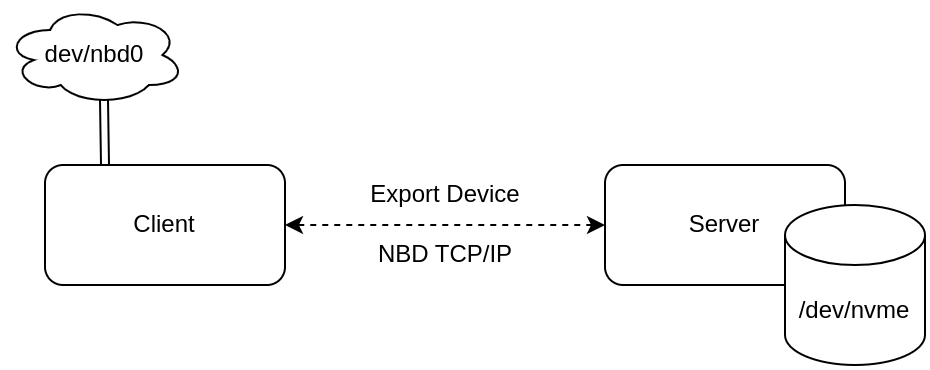
\includegraphics[scale=0.22]{figures/nbd-path.png}\\
    \caption{Overview of an NBD system.}
    \label{fig:nbd_path}
  \end{figure}
\par The nbd-client usually resides in the OS kernel and exposes a block device interface to the rest of the kernel, so that it may appear as an ordinary, directly-attached storage device. The client passes the block requests to the NBD driver where they are encapsulated as NBD network messages and sent to the server via TCP. Finally the User-Space server upon receiving the NBD request issues standard I/O to the relevant block device and then responds Figure \ref{fig:nbd_path2} shows a more in depth I/O path using NBD TCP Version.
 There are multiple NBD implementations, including:
 \begin{itemize}
 \item  \textbf{nbdkit} is a multi-threaded NBD server with a plugin architecture.
 \item  \textbf{libnbd} is a library to aid in writing NBD clients.
 \item  \textbf{qemu} contains an \textbf{embedded NBD server}, \textbf{an embedded NBD client}, and \textbf{a standalone NBD server} (qemu-nbd). They maintain a status document of their NBD implementation.
 \item  A \textbf{GEOM gate-based client implementation for FreeBSD} exists. It has not seen any updates since 2018, and only implements the client side (any server should run on FreeBSD unmodified, however).
 \item  A \textbf{Windows} client implementation exists as part of the RBD implementation of Ceph for Windows.
 \item  \textbf{lwNBD} is a NBD server library, targetting bare metal or OS embedded system. It has a plugin architecture.
 \end{itemize}
 We will focus on the Network Block Device (TCP version) ~\cite{nbd}. We use the TCP version to investigate the overheads added by the TCP protocol stack and compare it with other mechanisms for exporting block devices over the network. With this implementation compiled in the kernel we can use 2 drivers/modules, the nbd-client and the nbd-server. 
\begin{figure}[h]
    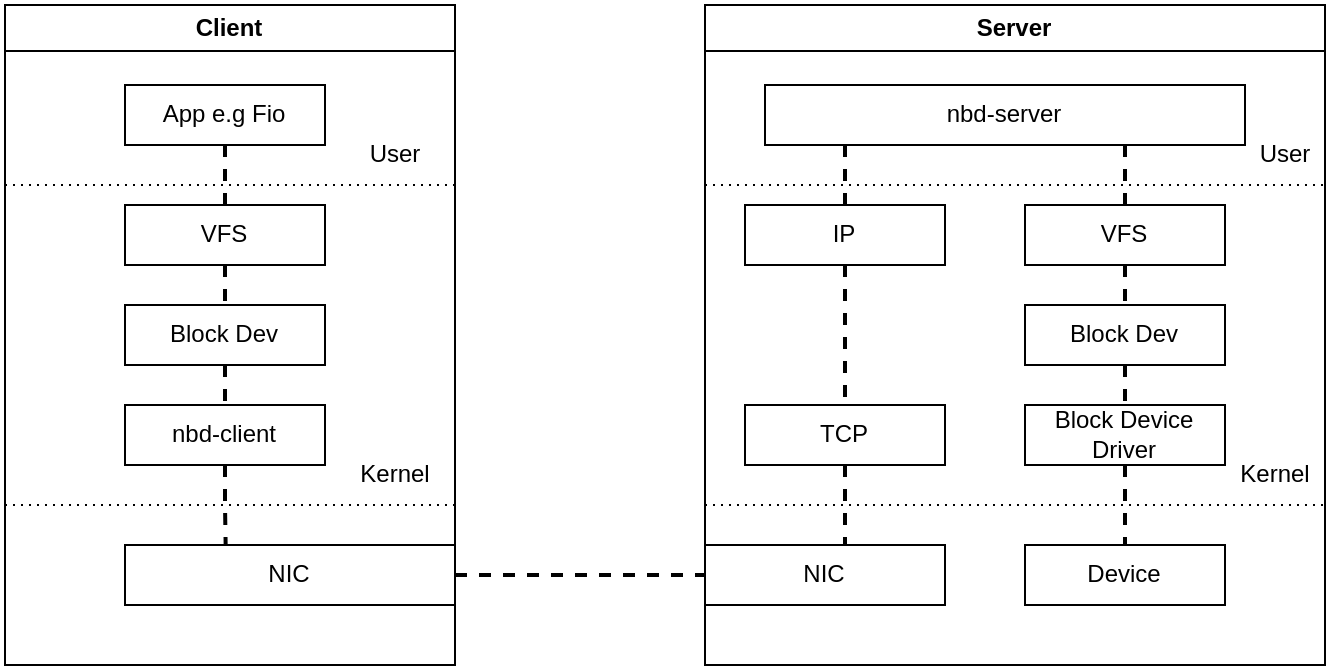
\includegraphics[scale=0.18]{figures/nbd-path2.png}\\
    \caption{I/O Path of NBD system.}
    \label{fig:nbd_path2}
  \end{figure}

\subsection{NVMe over Fabrics (NVMe-oF)}
NVMe over Fabrics (NVMe-oF) ~\cite{nvme-of} is a protocol specification designed for connecting
hosts to storage systems over a network using the NVMe protocol. It enables the
transfer of data between a host computer and a target solid-state storage device
or system through network communication. This protocol utilizes NVMe
message-based commands to facilitate data transfers, supporting various
networking technologies such as Ethernet, Fibre Channel (FC), and InfiniBand.

\subsection{Storage Performance Development Kit (SPDK)}
The Storage Performance Development Kit (SPDK) ~\cite{spdk} is a versatile toolkit tailored
for crafting high-performance, scalable storage applications in user-mode
environments. Its architecture revolves around several core principles aimed at
optimizing performance like User-Space Drivers, Polling Mechanism and lockless
I/O handling. At its foundation, SPDK features a user-space, asynchronous NVMe
driver designed for zero-copy, highly parallel access to SSDs. This driver,
presented as a C library with a simple public header, facilitates seamless
integration for developers. Additionally, SPDK offers a user-space block stack
library mirroring OS functionalities, including storage device interface
unification, queue management for resource constraints, and logical volume
administration. SPDK extends its capabilities with NVMe-oF, iSCSI, and vhost
servers built atop these foundational components. 

\par SPDK operates entirely in user space, bypassing the kernel entirely for I/O operations. By eliminating the overhead of kernel context switches and system calls, SPDK can achieve significantly higher performance and lower latency compared to traditional storage solutions that rely on kernel-level operations. Memory management in SPDK is highly optimized, utilizing techniques such as large memory buffers, memory pooling, and zero-copy operations. Large memory buffers are allocated upfront, often using huge pages, to ensure contiguous memory allocation and reduce fragmentation. Memory pooling minimizes the overhead of dynamic memory allocation and deallocation, while zero-copy operations eliminate unnecessary data copies, further enhancing performance. Integration with the Data Plane Development Kit (DPDK) enhances SPDK's performance by leveraging DPDK's ~\cite{dpdk} efficient packet processing capabilities for networked storage solutions. This integration enables SPDK to handle network I/O with minimal overhead, ensuring high throughput and low latency for storage applications deployed in networked environments. SPDK's support for NVMe-oF extends the NVMe protocol over fabrics, allowing remote access to NVMe storage devices with minimal overhead. This involves sophisticated handling of NVMe commands and data over high-speed networks, optimizing performance and scalability for distributed storage solutions.
\begin{figure}[H]
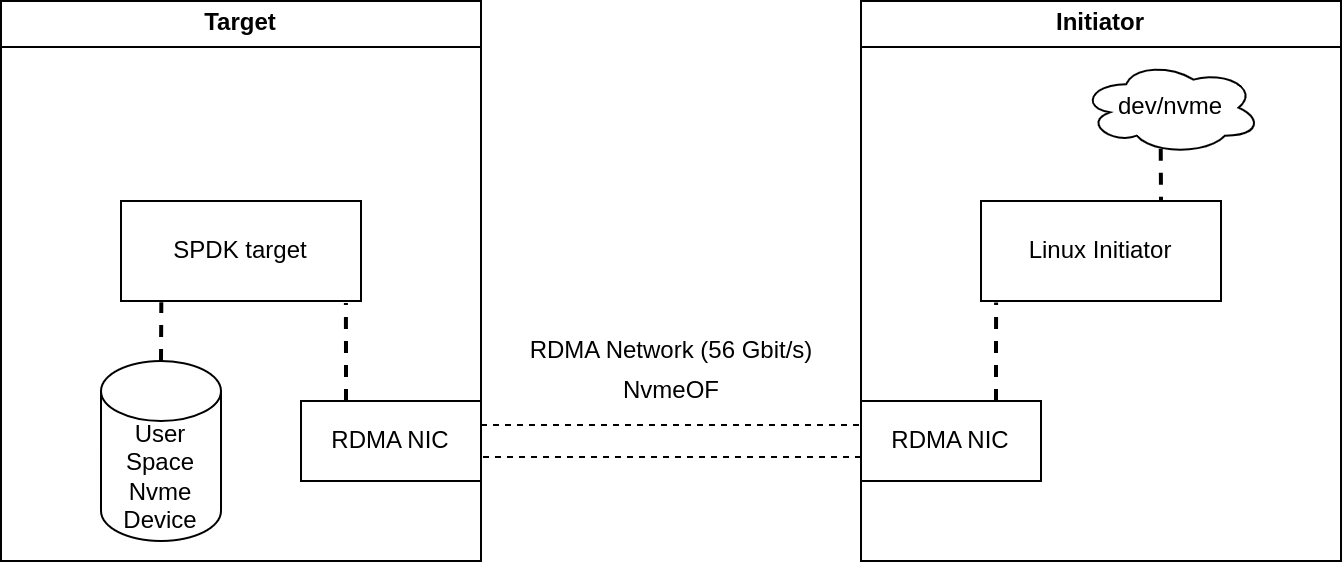
\includegraphics[scale=0.18]{figures/spdk-target.png}\\
\caption{Overview of SPDK NvmeOF Target-Initiator system.}
\label{fig:spdk}
\end{figure}
\par Figure \ref{fig:spdk} Shows an overview of the SPDK NVMe-oF Target-Initiator system. The process begins with the target unbinding traditional kernel drivers associated with the block device and binding them with SPDK's user-space drivers. This step grants SPDK exclusive control over the block device, enabling optimized I/O handling and performance. Subsequently, the block device, now under the control of SPDK in user space, is exported to the network using the NVMe-oF protocol specification, facilitated by RDMA. RDMA plays a pivotal role in enabling high-speed, low-latency data transfers over the network, allowing direct access to remote system memory without CPU involvement. This process ensures efficient data transmission between the NVMe target and initiator. Additionally, SPDK supports kernel initiators, allowing traditional kernel-based applications to connect to SPDK NVMe-oF targets. Through this mechanism, kernel initiators can access the SPDK-exported block device over the network using standard device nodes such as /dev/nvme.